\documentclass[thesis.tex]{subfiles}
\chapter{Nhận dạng người nói tiếng Việt}
Trong chương này, tác giả trình bày phương pháp học sâu để giải quyết bài toán nhận diện người nói. Ngoài ra tác giả cũng đề xuất phương pháp để cải tiến mô hình hiện tại để đạt được kết quả cao hơn trên tiếng Việt.

\section{Hệ thống cơ sở}
Hệ thống tác giả sử dụng trong đồ án tuân theo hệ thống ba pha được mô tả như trong \ref{related-works}, đây là sự kết hợp giữa mô hình ResNet, lớp tổng hợp thống kê tập trung (attentive statistic pooling - ASP) và hàm mất mát Angular Prototypical (AP). Kiến trúc của hệ thống được miêu tả trong Hình \ref{fig:ap-resnet}. 

\begin{figure}[h]
    \centering
    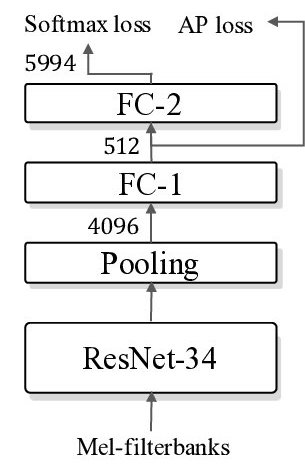
\includegraphics[width=0.4\textwidth]{images/ap-resnet.jpg}
    \caption{Tổng quan hệ thống sử dụng hàm mất mát Angular Prototypical}
    \label{fig:ap-resnet}
\end{figure}

Đầu vào của hệ thống là \TODO{...}.

Trong các mục tiếp theo, tác giả sẽ trình bày chi tiết thành phần của hệ thống.

\subsection{Biểu diễn khung âm thanh bằng mạng ResNet}
Đầu vào của mạng ResNet là 

\subsection{Tổng hợp thống kê tập trung}
Trong thực tế, không phải khung âm thanh nào cũng chứa nhiều thông tin của người nói do độ dài một khung rất ngắn thông thường chỉ 25 mili giây. Ví dụ, một khung có thể chứa nhiều tiếng ồn, hoặc không hề chứa giọng nói. Do vậy, hệ thống sử dụng tổng hợp thống kê tập trung để đánh trọng số cho biểu diễn của các khung với mong muốn tăng thông tin của những khung nhiều ý nghĩa và giảm thông tin của những khung ít ý nghĩa. Từ đó có thể phân biệt giọng nói một cách hiệu quả hơn.

% Được đề xuất bởi Okabe và cộng sự trong \cite{okabe2018attentive}, tổng hợp thống kê tập trung là sự kết hợp giữa tổng hợp thống kê \cite{snyder2018x} và cơ chế tập trung (attention mechanism) \cite{raffel2015feed}.

ASP nhận đầu vào là tập các vec-tơ biểu diễn khung $\bm{h}_t\ (t=1,...,T)$. Vec-tơ biểu diễn của toàn đoạn âm thanh được tính qua 2 bước: đánh trọng số cho từng khung bằng cơ chế tập trung và tổng hợp thông tin thống kê dựa trên trọng số tính được.

\subsubsection{Cơ chế tập trung}

Bằng cơ chế tập trung, trọng số của từng khung có thể được tính như sau: 

\begin{equation} \label{eq:att1}
    e_t = \bm{v}^T f(\bm{W}\bm{h}_t + b) + k
\end{equation}

\begin{equation} \label{eq:att2}
    \alpha_t = \dfrac{\alpha_t}{\sum_\rho^T \alpha_\rho}
\end{equation}

Trong công thức \ref{eq:att1}, với $\bm{v}, \bm{W}$ là các ma trận trọng số có thể học được, $f$ là hàm phi tuyến như thanh hoặc ReLu, ta tính được điểm cho mỗi khung $e_t$. Sau đó, điểm của mỗi khung được chuẩn hoá trên tất cả các khung để thu được trọng số tập trung bằng hàm softmax như trong \ref{eq:att2}.

\subsubsection{Tổng hợp thống kê}
Sau khi có được trọng số của các khung, ta tính vec-tơ trung bình có trọng số:

\begin{equation} \label{eq:asp1}
    \bm{\mu} = \sum_t^T \alpha_t\ \bm{h}_t
\end{equation}

Bằng cách tính này, vec-tơ biểu diễn của đoạn âm thanh tập trung hơn vào những khung tiếng nói có ý nghĩa cao. Ngoài ra, các trọng số tập trung còn được sử dụng để tính độ lệch chuẩn có trọng số:

\begin{equation} \label{eq:asp2}
    \bm{\sigma} = \sqrt{\sum_t^T \alpha_t \bm{h}_t \odot \bm{h}_t - \bm{\mu} \odot \bm{\mu}}
\end{equation}

Với $\odot$ là phép nhân Hadamard, $\bm{\mu}$ là vec-tơ trung bình có trọng số tính trong công thức \ref{eq:asp1}. Sau khi hoàn tất quá trình tính toán vec-tơ trung bình và độ lệch chuẩn có trọng số, $\bm{\mu}$ và $\bm{\sigma}$ được ghép lại để biểu diễn cho một đoạn tiếng nói. Bằng cách này, mọi đoạn âm thanh dài ngắn đều có vec-tơ biểu diễn với số chiều như nhau, được tổng hợp từ những khung âm thanh có ý nghĩa nhất trong câu.

\subsection{Hàm mất mát Angular Prototypical}
Trong thực tế, ta cần tổng hợp từ một số câu nói nhất định để tạo vec-tơ biểu diễn người nói. Do vậy, Chung và cộng sự \cite{chung2020defence} đề xuất hàm mất mát AP tối ưu không gian biểu diễn dựa trên nguyên mẫu (prototype) của người nói. Mỗi người nói có một nguyên mẫu và một câu truy vấn, mục tiêu của AP là đẩy xa truy vấn của một người ra xa nguyên mẫu của những người khác và kéo nó lại gần nguyên mẫu của người đó (Hình \ref{fig:ap-loss}).

\begin{figure}[h]
    \centering
    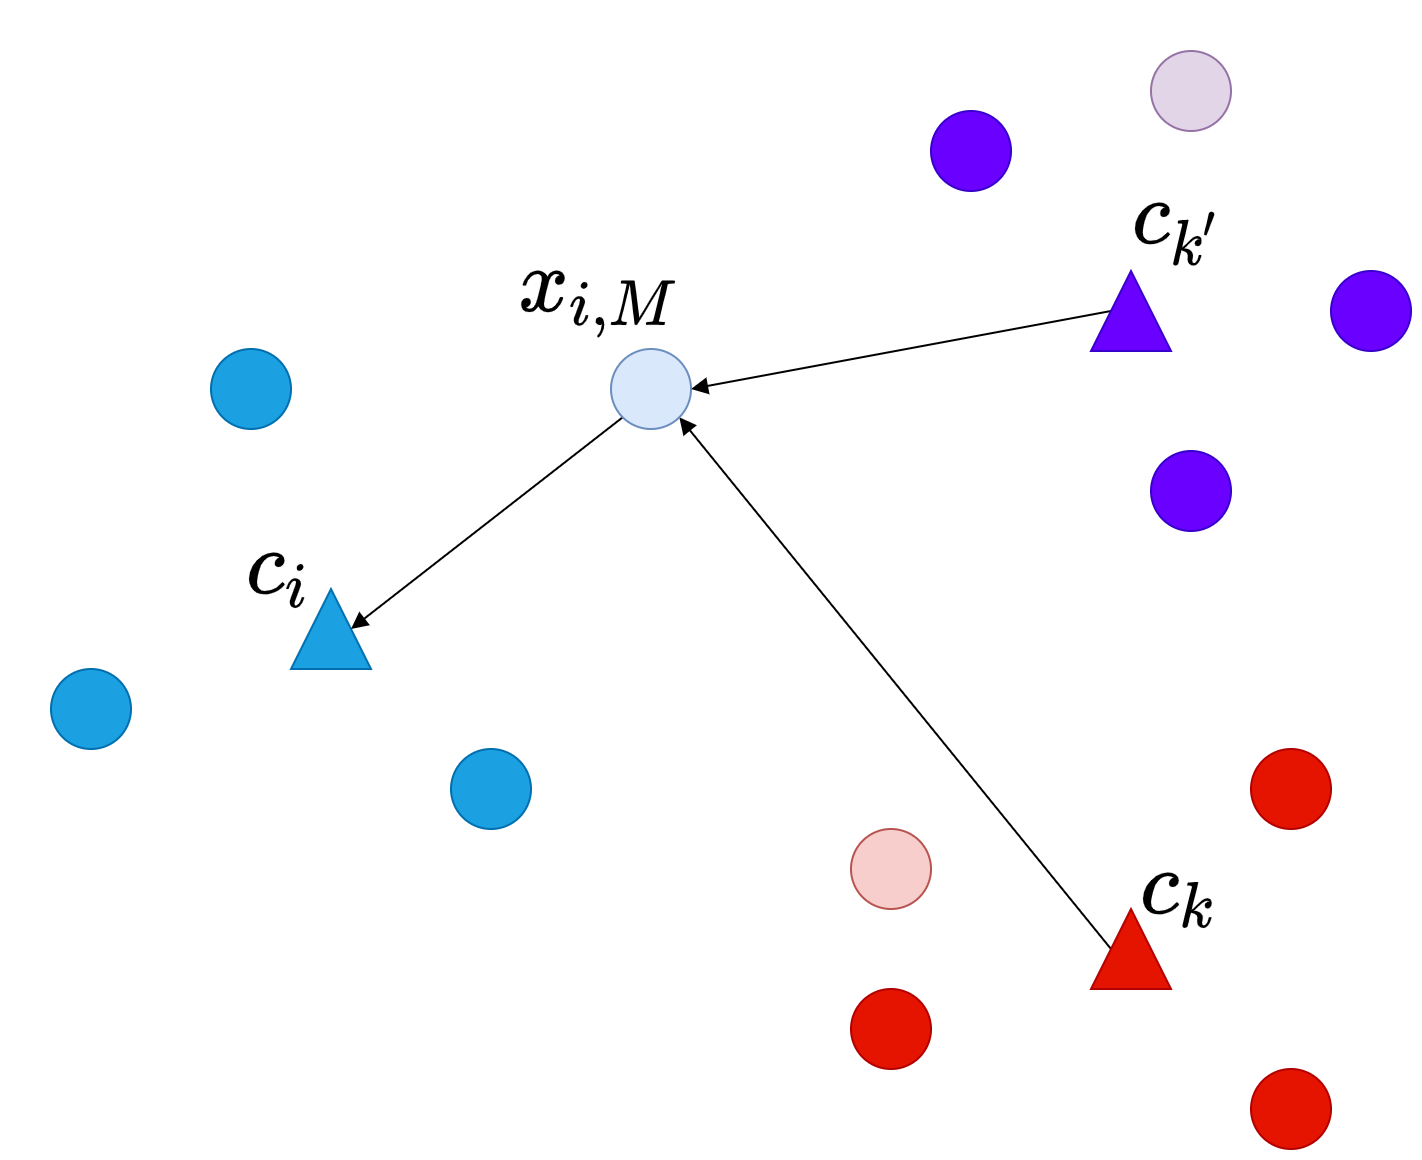
\includegraphics[width=0.7\textwidth]{images/ap-loss.png}
    \caption{Hàm mất mát Angular Prototypical}
    \label{fig:ap-loss}
\end{figure}

Xét một mini-batch gồm $M$ đoạn tiếng nói từ mỗi $N$ người nói, gọi $\bm{x}_{i,j}$ là vec-tơ biểu diễn của đoạn tiếng nói thứ $j$ của người thứ $i$, $1 \leq i \leq N, 1 \leq j \leq M$. Giả sử truy vấn của một người là câu cuối cùng của người đó $\bm{x}_{i,M}$, nguyên mẫu của một người nói được tính toán như sau:

\begin{equation}
    \bm{c}_i = \dfrac{1}{M-1}\sum_{m=1}^{M-1}\ \bm{x}_{i,m}
\end{equation}

Trong AP, độ tương đồng cô-sin được sử dụng để làm độ đo. Độ tương đồng được tính theo công thức \ref{eq:cosine} với hệ số scale $w$ và bias $b$. Hai hệ số này giúp mô hình hội tụ ổn định hơn và khái quát hoá tốt hơn với thay đổi trong đặc trưng đầu vào \cite{wang2017deep}.

\begin{equation}\label{eq:cosine}
    \bm{S}_{i,k} = w \cdot cos(\bm{x}_{i,M}, \bm{c}_k) + b
\end{equation}

Trong quá trình huấn luyện, câu truy vấn của mỗi người được phân loại dựa trên độ tương đồng đối với $N$ nguyên mẫu trong mini-batch:

\begin{equation}\label{eq:nll-softmax}
    L_P = - \dfrac{1}{N} \sum_{i=1}^N log \dfrac{e^{\bm{S}_{i,i}}}{\sum_{k=1}^N e^{\bm{S}_{i,k}}}
\end{equation}

Trong công thức \ref*{eq:nll-softmax}, $\bm{S}_{i, i}$ là độ tương đồng của truy vấn người $i$ và nguyên mẫu của chính người đó. Bằng việc sử dụng hàm softmax, $\bm{S}_{i,i}$ được đẩy gần hơn tới 1 và mô hình bị "phạt" nặng hơn nếu độ tương đồng của truy vấn người $i$ tới nguyên mẫu của người khác lớn.

\section{Đề xuất cải tiến mô hình}
Trong phần này, đề xuất ... 

\subsection{Transfer learning}
Transfer learning là một kỹ thuật trong học máy khi mà một mô hình được huấn luyện cho một tác vụ nhất định được sử dụng làm điểm bắt đầu cho một tác vụ khác. Transfer learning cho phép rút ngắn quá trình huấn luyện và gia tăng hiệu năng cho quá trình huấn luyện mô hình trên tác vụ mới với ít dữ liệu hơn đáng kể. 

\begin{figure}[h]
    \centering
    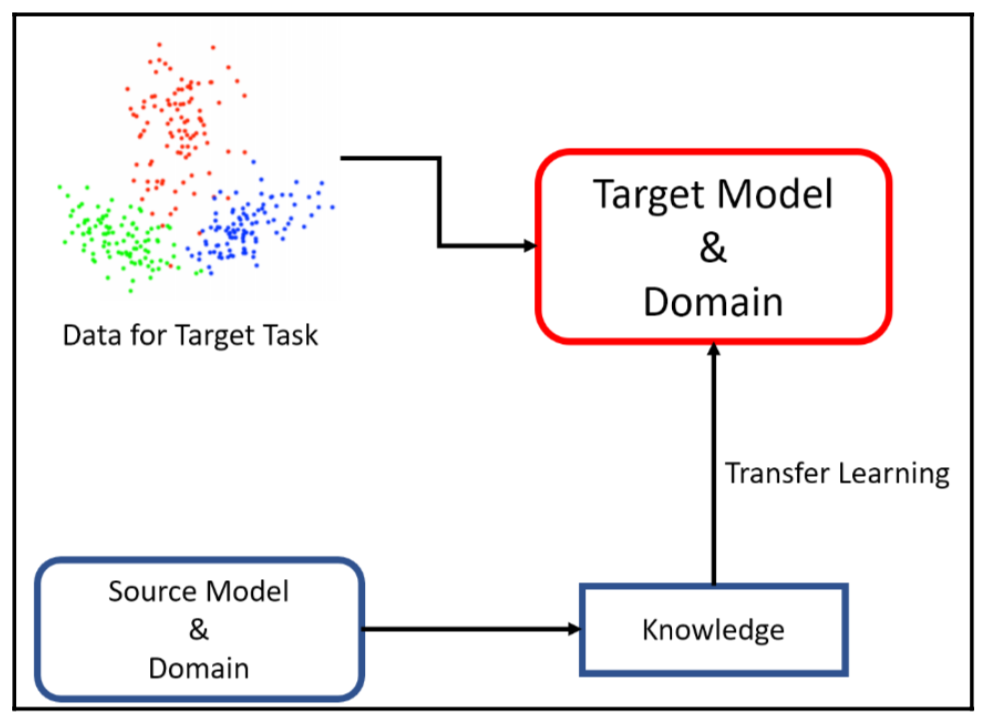
\includegraphics[width=0.7\textwidth]{images/transfer-learning.png}
    \caption{Sơ đồ mô tả transfer learning sử dụng kiến thức hiện có cho các tác vụ mới \cite{sarkar2018hands}}
    \label{fig:transfer-learning}
\end{figure}

Cụ thể hơn, transfer learning hỗ trợ việc huấn luyện tác vụ mục tiêu theo những cách sau: 

\begin{itemize}
    \item Hiệu suất cơ sở tốt hơn (higher start): khi ta tăng cường kiến thức của mô hình mới với kiến thức từ mô hình gốc, hiệu suất cơ sở có thể cải thiện nhờ việc chuyển giao kiến thức.
    \item Thời gian huấn luyện ngắn hơn (higher slope): tốc độ hội tụ của mô hình mới có thể nhanh hơn dẫn tới thời gian huấn luyện ngắn hơn.
    \item Kết quả cuối cùng tốt hơn (higher asymptote): hiệu suất cuối cùng cao hơn có thể đạt được bằng việc sử dụng transfer learning.
\end{itemize}

\begin{figure}[h]
    \centering
    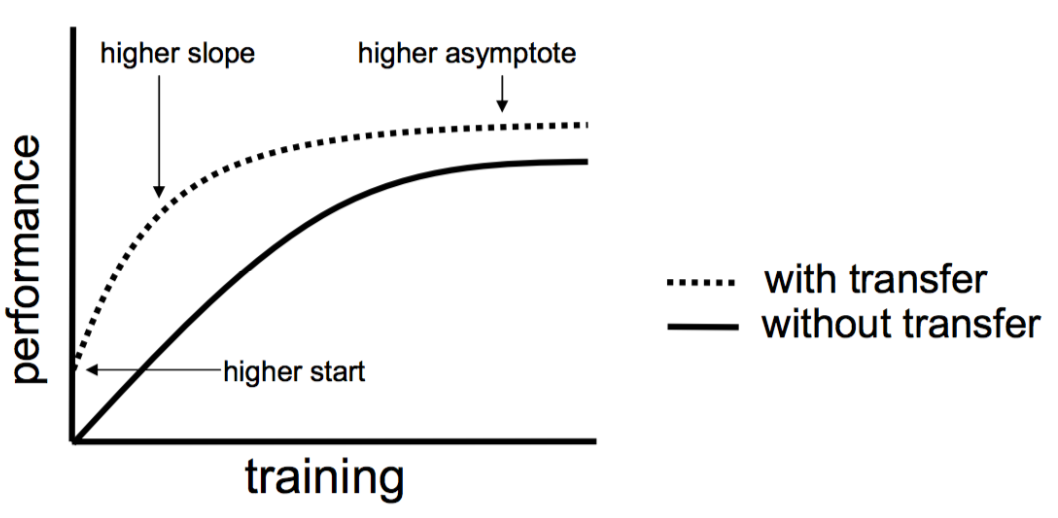
\includegraphics[width=0.7\textwidth]{images/transfer-learning-benefits.png}
    \caption{Lợi ích của transfer learning đối với việc huấn luyện mô hình \cite{aytar2011tabula}}
    \label{fig:transfer-learning-benefits}
\end{figure}

Huấn luyện mô hình học sâu cần một lượng lớn tài nguyên tính toán và dữ liệu, do đó transfer learning được sử dụng rộng rãi trong cộng đồng nghiên cứu học sâu cho bài toán thị giác máy tính hay xử lý ngôn ngữ tự nhiên. \TODO{...}

\subsection{Stochastic gradient descent khái quát hoá tốt hơn ADAM}
\subsection{Angular margin tăng khoảng cách giữa các người nói trong không gian embedding}
% https://medium.com/analytics-vidhya/exploring-other-face-recognition-approaches-part-2-arcface-88cda1fdfeb8
% https://medium.com/analytics-vidhya/exploring-other-face-recognition-approaches-part-1-cosface-4aed39afe7a8